\documentclass[fontsize=10pt,DIV=14]{scrartcl}

\usepackage{enumitem}
	\setenumerate{listparindent=\parindent}
\usepackage{amsmath}
\usepackage{amssymb}
\usepackage{graphicx}
\usepackage{placeins}
\usepackage{hyperref}
\usepackage{float}
\usepackage{tabularx}
\usepackage{listings}

\newcommand{\code}{\texttt}

\begin{document}

	\title{CSC 522 : Automated Learning and Data Analysis}
	\subtitle{Homework 5}
	\author{Roopak Venkatakrishnan - rvenkat7@ncsu.edu}
	\maketitle

	\section{Question 1 [57 Points (25 + 32)] - Regression}

	In this problem we will investigate various methods for fitting a linear model for regression. Download the regprob.zip file from the course website.

	\begin{enumerate}
		\item
		Given a set of n real-valued responses $y_{i}$ and a set of p predictors, we might try to model $y_{i}$ as a linear combination of the p predictors. The form of this type of linear model is:
		\begin{equation*}
			y_{i} = \beta_{0} +\sum_{j=1}^{p} + \beta_{j} \times x_{ij}
		\end{equation*}

		where $y_{i}$ is the the value of the response for the $i^{th}$ observation, $x_{ij}$ is the value for the $j^{th}$ predictor for observation i, and $\beta_{0}$ is the intercept. To find ’good’ values for all of the $\beta$s, one approach is to minimize the sum of squared errors (SSE), shown below:

		\begin{equation*}
			SSE =\sum_{i=1}^{n} (y_{i} - \beta_{0} - \sum_{j=1}^{p} \beta_{j} \times x_{ij})
		\end{equation*}

		This approach is known as regression via ordinary least squares (OLS). Representing this model in matrix notation, the model can be written in an equivalent form as $Y = X\beta$. Now Y is an $n \times 1$ column vector containing the response variable, X is an $n \times (p + 1)$ matrix that contains the $p$ predictors for all $n$ observations as well as a column of all 1s to represent the intercept, and $\beta$ is a $p + 1$ vector. With some matrix calculus it can be shown the value of $\beta$ that minimizes the SSE is given by:

		\begin{equation*}
			\hat{\beta}_{OLS} = (X^{T} X)^{-1} X^{T}Y
		\end{equation*}

		where $T$ indicates a matrix transpose. This formula will give a $(p + 1)$ vector containing the estimated regression coefficients.

		Complete the following tasks:
		\begin{itemize}
			\item
			Load \emph{train.csv}

\begin{verbatim}
> train <- read.csv(file.choose())
\end{verbatim}
			
			\item
			Compute the OLS estimates using the data in train.csv. Do not use a package to do this, instead compute it directly from the formula given above. There are 10 predictors in the file, so your solution should contain 11 estimated regression coeffcients (1 for each predictor plus 1 for the intercept, 11 numbers in total).

			\begin{lstlisting}[language=R,frame=single]
> library(caret)
Loading required package: cluster
Loading required package: foreach
foreach: simple, scalable parallel programming from Revolution Analytics
Use Revolution R for scalability, fault tolerance and more.
http://www.revolutionanalytics.com
Loading required package: lattice
Loading required package: plyr
Loading required package: reshape2
> x_data <- train[2:11]
> y_data <- train[1]
> X0 <- rep(1,100)
> x_data <- cbind(X0,x_data)
> xt <- t(x_data)
> xtx <- as.matrix(xt) %*% t(xt)
> xty <- as.matrix(xt) %*% as.matrix(y_data)
> beta <- solve(xtx) %*% xty
> beta
                Y
X0   2.0011897376
X1   1.4866088726
X2  -1.9616801211
X3   3.0082822263
X4   1.7619676828
X5  -0.4978060382
X6  -0.0319859478
X7   0.0120974698
X8  -0.0006889951
X9  -0.0060084271
X10  0.0112536257
			\end{lstlisting}
			\textbf{Note:} In the above case $X0$ is the coeffiecient of $\beta$ for the intercept
			\item
			Estimate the mean squared error on an unseen test set by performing 5-fold crossvalidation. Recall the MSE for a set of $y$ observations and $\hat{y}$ predictions is defined as
			\begin{equation*}
				MSE = \frac{1}{N} \sum_{i=1}^{n} (y_{i} - \hat{y_{i}})^{2}
			\end{equation*}

			\begin{lstlisting}[language=R,frame=single]
> folds2 <-createFolds(train[["Y"]],k=5,list=FALSE)
> mse <- rep(0,5)
> for(i in 1:5) {  
+  
+   fold.rows <- which(folds2 == i)
+   cv.train <- train[-fold.rows,]
+   
+   cv.test <- train[fold.rows,]
+   
+   x_train <- cv.train[2:11]
+   y_train <- cv.train[1]
+   X0 <- rep(1,80)
+   x_train <- cbind(X0,x_train)
+   xt <- t(x_train)
+   xtx <- as.matrix(xt) %*% t(xt)
+   xty <- as.matrix(xt) %*% as.matrix(y_train)
+   beta <- solve(xtx) %*% xty
+   
+   x_test <- cv.test[2:11]
+   y_act <- cv.test[1]
+   xpred <-  mapply("*",t(beta)[2:11],x_test)
+   xpred <- cbind(t(beta)[1],xpred)
+   y_pred <- rowSums(xpred)
+   ydiff <- cbind(y_act,y_pred)
+   ydiff$diff <- ydiff$Y - ydiff$y_pred
+   yd_sq <- ydiff$diff^2
+   mse[i] <- sum(yd_sq)/20
+ }
> mse
[1] 0.03354157 0.04317550 0.06382128 0.03696788 0.04751039
> mean(mse)
[1] 0.04500332
			\end{lstlisting}

			We get the Mean MSE to be $0.04500332$.
		\end{itemize}

		\item
		The term `linear model' indicates that a model is linear with respect to $\beta$. However, we can model higher order polynomial terms by explicity computing them, including them in the $X$ matrix, and then fit a linear model to this matrix. Perform the following tasks:

		\begin{itemize}
			\item
			Load \emph{polynomial.train.csv}
			\begin{verbatim}
> data <- read.csv(file.choose())
			\end{verbatim}

			\item
			Plot $Y$ as a function of $X$
\begin{verbatim}
> plot(data[["X"]],data[["Y"]],xlab="X data",ylab="Y data")
\end{verbatim}
			
			\begin{figure}[H]
				\begin{center}
					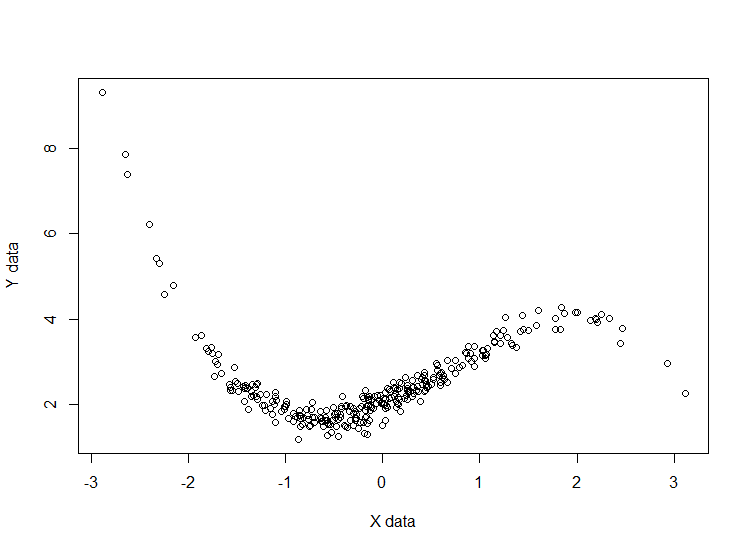
\includegraphics[width=\textwidth]{resources/q1_2_img1.png}
					\caption{Plot with points}
				\end{center}
			\end{figure}
			\item
			Create a new $X$ matrix that includes a column of 1s for an intercept, a column for the original $X$ values, and a column of polynomials for each $X^{i}$ for $i \in {2,3,4,5}$. This will create a matrix with dimensions $300 \times 6$.
			\begin{verbatim}
> x_data <- cbind(rep(1,300),data["X"],data["X"]^2,data["X"]^3,data["X"]^4,data["X"]^5)
> names(x_data) <- c("X0","X1","X2","X3","X4","X5")
			\end{verbatim}

			\item
			Find the OLS solution to this using $(X^{T}X)^{-1} X^{T}Y$.

\begin{lstlisting}[language=R,frame=single]
> xt <- t(x_data)
> xtx <- as.matrix(xt) %*% t(xt)
> xty <- as.matrix(xt) %*% as.matrix(data["Y"])
> beta <- solve(xtx) %*% xty
> beta
               Y
X0  2.0142724145
X1  0.9522479087
X2  0.5014464975
X3 -0.2219555459
X4  0.0001422326
X5 -0.0031247916
\end{lstlisting}
		\textbf{Note:} Here $X0$ is the intercept while $X1,X2,X3,X4,X5$ denote powers of $X$ etc.

		\item
		Overlay the fitted values (i.e. $X\hat{\beta}_{OLS}$) as a line on the plot of $Y$ vs. $X$.
		\begin{lstlisting}[language=R,frame=single]
> xpred <-  mapply("*",t(beta),x_data)
> y_pred <- rowSums(xpred)
> pred<- cbind(y_pred,x_data[2])
> pred_out <- arrange(pred,X1)
> plot(data[["X"]],data[["Y"]],xlab="X data",ylab="Y data")
> lines(pred_out$X1,pred_out$y_pred,col="red")
		\end{lstlisting}
		\begin{figure}[H]
				\begin{center}
					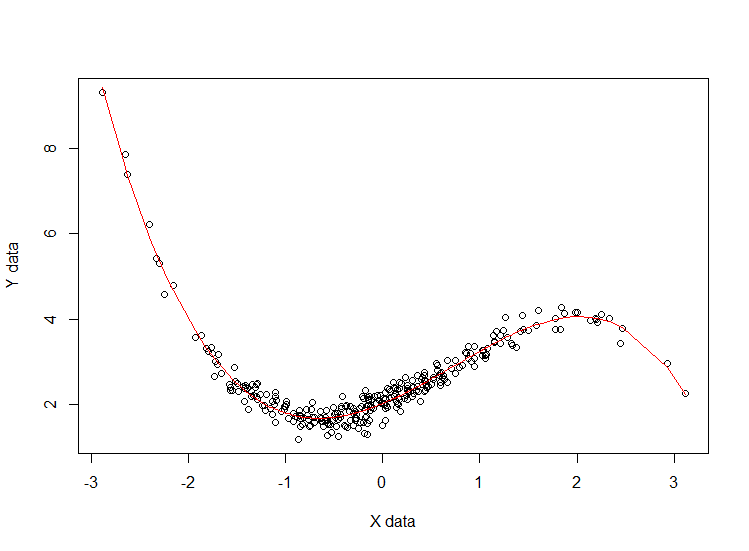
\includegraphics[width=\textwidth]{resources/q1_2_img2.png}
					\caption{Plot with points and overlaid line}
				\end{center}
			\end{figure}
		\end{itemize}
	\end{enumerate}
\end{document}